\documentclass{beamer}

\usetheme{Antibes}
\usepackage{pgfplots}
\usepackage{graphicx}
\title[Laxman]{Q.no. 19 in GATE ECE 2015  }
\subtitle{Control Systems}
\author{Sai Laxman-EE18BTECH11049}


\begin{document}

\begin{frame}
\titlepage    
\end{frame}



\section{Question}


\begin{frame}{ Question}
Negative Feedback in a closed-loop control system $DOES$ $ NOT ?$\\

  a.)Reduce overall gain\\
  b.)Reduce sensitivity to parameter variation\\
  c.)Improve disturbance rejection \\
  d.)Reduce bandwidth\\
  
\end{frame}





\section{Solution}




\begin{frame}{Solution : Option-a }

\begin{figure}
    \resizebox{.6\columnwidth}{!}{%\begin{figure}
\tikzstyle{block} = [draw, fill=blue!20, rectangle, 
    minimum height=0.7cm, minimum width=0.7cm]
\tikzstyle{sum} = [draw, fill=blue!20, circle, node distance=1cm]
\tikzstyle{input} = [coordinate]
\tikzstyle{output} = [coordinate]
\tikzstyle{pinstyle} = [pin edge={to-,thin,black}]

\begin{tikzpicture}[auto, node distance=2.5cm,>=latex]
    % We start by placing the blocks
    \node [input, name=input] {};
    \node [sum, right of=input] (sum) {};
    \node [block, right of=sum] (controller) {G(s)};
    \node [output, right of=controller] (output) {};
    \node [block, below of=controller] (measurements) {H(s) =  $\beta$ };

    \draw [draw,->] (input) -- node {$X(s)\  +$} (sum);
    \draw [->] (sum) -- node {} (controller);
    \draw [->] (controller) -- node [name=y] {$Y(s)$}(output);
    \draw [->] (y) |- (measurements);
    \draw [->] (measurements) -| node[pos=0.99] {$-$} 
        node [near end] {$Z(s)$} (sum);
\end{tikzpicture}
%\end{figure}

}
\end{figure}

\begin{align}
\text{Closed loop gain }
 Y(s)/X(s) = \frac {\mid G(s) \mid}{ \mid 1+\beta G(s) \mid}
 \label{eq:ee18btech11049_closed_loop_gain}
\end{align}
\begin{align}
  \text{ Open loop gain =}  \mid G(s) \mid
  \label{eq:ee18btech11049_open_loop_gain}
\end{align}
\begin{align}
    Comparing \eqref{eq:ee18btech11049_closed_loop_gain} and \eqref{eq:ee18btech11049_open_loop_gain} 
\end{align}

\end{frame}


\begin{frame}{Option-a }

\begin{align}
    \mid1+\beta H(s)\mid  > 1
\end{align}
\begin{align}
    \frac{1}{\mid1+\beta H(s)\mid}  < 1
\end{align}
\begin{align}
    \frac{\mid G(s) \mid}{\mid1+\beta H(s)\mid}  < \mid G(s) \mid
    \label{eq:ee18btech11049_proof_red}
\end{align}
from \eqref{eq:ee18btech11049_proof_red} we can say  - closed loop gain $<$ open loop gain
\end{frame}



\begin{frame}{Option-b}
Sensitivity to parameter variation :\\



\[     sensitivity 
  = \dfrac{change\ in\ overall\ gain}{change\ in\ system\ parameter}
\]




-- Lets take system parameter be G\\ 
\begin{align}
     \text{And closed loop Sensitivty}  = \frac{(dT/T*100)}{(dG/G*100)}  = \frac{1}{1+GH}
\end{align}

\begin{align}
\text{ open loop Sensitivity }= 1 
\end{align}
Therefore, reduced sensitivity.



\end{frame}

\begin{frame}{Option -c}
    The use of feedback is to remove disturbance. As the output gets changed subsequently the input will be altered through feedback terminal .Thus, reducing the disturbance. \\
    
    Therefore, It improves disturbance Rejection.
\end{frame}{}






\begin{frame}{Option d bandwidth}
With 3db(Half power) frequency we can measure bandwidth of the system.

\begin{align}
   \text{ Power gain} = \mid H(jw) \mid ^2 =  \frac{\mid Y(jw) \mid ^2}{\mid X(jw) \mid ^2 }  
\end{align}
evaluating the magnitude squared at the "center" of  passband .\\
Taking w = 0 as center of passband.

\begin{align}
   \text{Open loop 3db }  \implies \mid H(jw) \mid ^2 =  \frac{1}{2}\mid H(0) \mid ^2
\end{align}
\begin{align}
   \text{Closed loop 3db } \implies \frac{\mid H(jw) \mid ^2}{\mid 1 + H(jw) \mid^2} =  \frac{1}{2}\frac{\mid H(0) \mid ^2}{\mid 1 + H(0) \mid^2}
\end{align}
\end{frame}



\begin{frame}{Option d}
considering positive half(w) and calculating values of H(jw):

\begin{align}
   \text{Open loop 3db }  \implies  H(jw)  =  \frac{1}{\sqrt{2}} H(0) 
\end{align}
\begin{align}
   \text{Closed loop 3db } \implies  H(jw) = \frac{H(0)}{\sqrt{2} + H(0)(\sqrt{2}-1)}
\end{align}

\begin{align}
  {H_{o}(jw) &= H_{c}(jw)}  
\end{align}
\begin{align}
  w_{o} < w_{c}  \text{   (As H(jw) is decreasing in positive half)}
\end{align}

Therefore bandwidth Increases.


\end{frame}



\begin{frame}
Proof : Plot for a system and its closed loop unity system.
\begin{figure}
    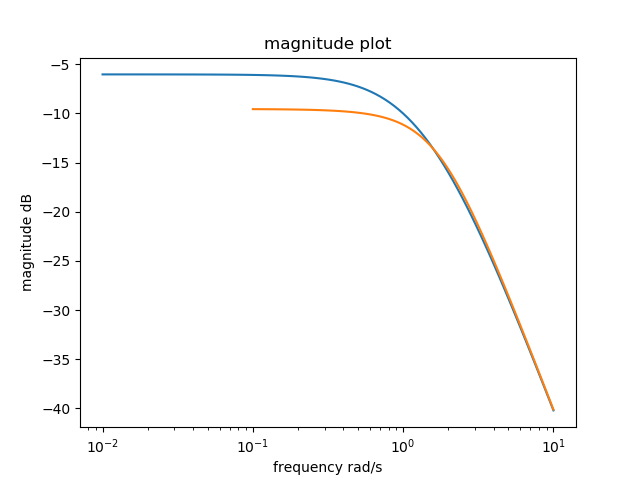
\includegraphics[scale=0.5]{plot2.png}
\end{figure}

From plot we can say bandwidth increases


\end{frame}


\end{document}
